\chapter{Mass fit to \decay{\Bp}{\Dsp\Kp\Km} candidates} 
\label{ch:B2DsKK}

\minitoc

In this chapter the methodology used to search for \decay{\Bp}{\Dsp\Kp\Km} decays is described.
The branching fraction $\BF(\decay{\Bp}{\Dsp\Kp\Km})$ is determined by measuring the ratio of \decay{\Bp}{\Dsp\Kp\Km} and \decay{\Bp}{\Dsp\Dzb} yields. 
This ratio is corrected to account for the corresponding selection efficiencies of the two modes. Finally, the corrected yield ratio is multiplied by the externally measured branching fractions for the normalisation channel \decay{\Bp}{\Dsp\Dzb} and \decay{\Dzb}{\Kp\Km} decays to determine $\BF(\decay{\Bp}{\Dsp\Kp\Km})$.


% This is corrected by the ratio of efficiencies for the two modes and multiplied by the externally measured branching fractions for \decay{\Bp}{\Dsp\Dzb} and \decay{\Dzb}{\Kp\Km} decays.

% \begin{multline}
% \BF(\decay{\Bp}{\Dsp\Kp\Km}) = \frac{N(\decay{\Bp}{\Dsp\Kp\Km})}{N(\decay{\Bp}{\Dsp\Dzb})} \times  \frac{\epsilon(\decay{\Bp}{\Dsp\Dzb})}{\epsilon(\decay{\Bp}{\Dsp\Kp\Km})}\\ 
% \times \BF(\decay{\Bp}{\Dsp\Dzb}) \times \BF(\decay{\Dzb}{\Kp\Km}) 
% \end{multline}

The parametrisations used to model the signal and backgrounds components and extract the candidate yields are described in Section~\ref{sec:B2DsKK_fitcomps}, the efficiency corrections are described in Section~\ref{sec:B2DsKK_effcorrection} and the resulting calculation of the branching fraction is in Section~\ref{sec:B2DsKK_results}.


\section{Fit components}
\label{sec:B2DsKK_fitcomps}

In order to extract the yields of \decay{\Bp}{\Dsp\Dzb} and \decay{\Bp}{\Dsp\Kp\Km} decays the invariant mass distributions for the processes contributing within the invariant mass range are parametrised with probability density functions (PDFs).
Both the signal and normalisation channels are considered within the same \Bp meson invariant mass range 5100--5900\mevcc. This is sufficiently wide to allow the contributions from different background components to be distinguished and accurately extrapolated into the signal region.  



\subsection{Signal and normalisation decays}
\label{sec:B2DsKK_sigcomps}

The invariant mass distribution of \decay{\Bp}{\Dsp\Dzb} and \decay{\Bp}{\Dsp\Kp\Km} decays are parametrised as the sum of two Crystal Ball (CB) functions.
The CB function consists of a Gaussian function with a power-law tail and is typically used to parametrise losses due to radiative processes.
This is defined as
\begin{equation}
\text{CB}(m|\mu,\sigma,n,\alpha) = \left \{
  \begin{aligned}
    &e^{-\frac{1}{2} \left(\frac{m-\mu}{\sigma}\right)^2}, && \text{if}\ \left(\frac{m-\mu}{\sigma}\right) < -|\alpha|\\
    &\frac{\left(\frac{n}{|\alpha|}\right)^n\times e ^{-\frac{1}{2}|\alpha|^2} }{\left(\frac{n}{|\alpha|}-|\alpha| - \frac{m-\mu}{\sigma}\right)^n}, && \text{otherwise}
  \end{aligned} \right.
\end{equation} 

where $\mu$, $\sigma$, $n$ and $\alpha$ are adjustable parameters and $m$ is the \B meson invariant mass observable.
The sum of two CB functions is constructed with a variable fraction $f_\sigma$ assigned to the CB function with the narrower width,
\begin{equation}
\text{DCB}(m|\mu,\sigma_1,\sigma_2,n,\alpha) = f_\sigma \times \text{CB}(m|\mu,\sigma_1,n,\alpha) + (1-f_\sigma) \times \text{CB}(m|\mu,\sigma_2,n,\alpha),
\label{eq:DoubleBD}
\end{equation}
where the same tail parameters, $n$ and $\alpha$ are used for both functions, but the widths, $\sigma_1$ and $\sigma_2$, are allowed to be different (with $\sigma_1 < \sigma_2$).
As both CB shapes have the same parameter $\alpha$, the tails are constrained to be on the same side.
Values for the adjustable parameters are determined from fits to simulated decays passing the selection requirements applied to the data. 
%These are determined separately for the different \Dsp decay modes. 
However, a number of parameters are not completely constrained from the simulations. The mean position $\mu$ is allowed vary freely in the fit to data, as is the narrowest CB width of the normalisation and signal decays. 
%The ratios $\sigma_1/\sigma_2$ and $\sigma_{1}(\Dsp\phi) / \sigma_{1}(\Dsp\Dzb)$ are fixed from simulations.
The tail parameters $n$ and $\alpha$ are highly correlated, therefore the value of $n$ is fixed to unity in both the fits to simulations and data. The values determined from simulations for \decay{\Bp}{\Dsp\Dzb} and \decay{\Bp}{\Dsp\Kp\Km} decays are tabulated in Table~\ref{tab:B2DsKK_signal_mc_fits} and the results of the corresponding fits are shown in Fig.~\ref{fig:B2DsKK_signal_fits}.


%%%%%%%%%%%%%%%%%%%%%%%%%%%%%%%%%%%%%%%%%%%%%%%%%%%%%%%%%% 
\begin{table}[h]
\centering 
\begin{tabular}{ c c }
\hline
Parameter                   & Value \\
\hline
\multicolumn{2}{c} {\decay{\Bp}{\Dsp\Kp\Km}}\\

\hline
$\sigma_1/\sigma_2$         & 0.53 $\pm$ 0.02  \\
$f_\sigma$                  & 0.87 $\pm$ 0.02  \\
$\alpha$                    & 2.60 $\pm$ 0.03  \\
$n$                         & 1 $\pm$ 0        \\
\hline
\multicolumn{2}{c} {\decay{\Bp}{\Dsp\Dzb}}\\
\hline
$\sigma_1/\sigma_2$         & 0.60 $\pm$ 0.03    \\
$f_\sigma$                  & 0.66 $\pm$ 0.12    \\
$\alpha$                    & 2.67 $\pm$ 0.12    \\
$n$                         & 1 $\pm$ 0          \\
\hline
\end{tabular} 
\caption{Fixed values obtained in fits to simulations used in the model for the signal and normalisation PDFs.} 
\label{tab:B2DsKK_signal_mc_fits}
\end{table}
%%%%%%%%%%%%%%%%%%%%%%%%%%%%%%%%%%%%%%%%%%%%%%%%%%%%%%%%%% 

%%%%%%%%%%%%%%%%%%%%%%%%%%%%%%%%%%%%%%%%%%%%%%%%%%%%%%%%%%
\begin{figure}[!h]
    \centering
    \begin{subfigure}[t]{1.0\textwidth}
        \includegraphics[width=0.48\textwidth]{figs/B2DsKK/Plot_Signal_Fit_All_B2DsKK_Ds2KKPi.pdf}
        \includegraphics[width=0.48\textwidth]{figs/B2DsKK/Plot_Signal_Fit_All_B2DsD0_Ds2KKPi.pdf}
    \end{subfigure}\\
    \caption{Invariant mass fits to signal (left) and normalisation (right) channel simulation samples.}
    \label{fig:B2DsKK_signal_fits}   
\end{figure}
%%%%%%%%%%%%%%%%%%%%%%%%%%%%%%%%%%%%%%%%%%%%%%%%%%%%%%%%%%


\subsection{Partially reconstructed backgrounds}
\label{sec:B2DsKK_partrecocomps}

Partially reconstructed decays are those in which the five final state particles combined in the signal mode are only a subset of a background mode's final state.
Decays of \bquark-hadrons can contribute at lower invariant masses below the signal peak when one or more the decay products have not been reconstructed. 
For decays to contribute within the fitted \Bp invariant mass window, the particle or particles that have not been reconstructed must be fairly low-momentum (soft) such that the invariant mass of the remaining particles is large.

\subsubsection{Backgrounds to the normalisation channel}

The low invariant mass region of the \Dsp\Dzb spectrum is populated by decays of \Bp mesons to combinations of \D and excited \D mesons. These \Dstarzb and \Dss mesons decay strongly to a ground state \Dzb or \Dsp meson and a soft pion or photon. The branching fractions for these decays are listed in Table~\ref{tab:dstar_BFs}.


%%%%%%%%%%%%%%%%%%%%%%%%%%%%%%%%%%%%%%%%%%%%%%%%%%%%%%%%%% 
\begin{table}[h]
\centering
\begin{tabular}{ l c }

\hline
Decay                           & Branching fraction \\ 
\hline
\decay{\Dstarzb}{\Dzb\Pgamma}   &   $(64.7\pm0.9)\%$ \\
\decay{\Dstarzb}{\Dzb\piz}      &   $(35.3\pm0.9)\%$ \\
\decay{\Dssp}{\Dsp\Pgamma}      &   $(93.5\pm0.7)\%$ \\
\decay{\Dssp}{\Dsp\piz}         &    $(5.8\pm0.7)\%$ \\
\hline

\end{tabular}  
\caption{Branching fractions for excited charm mesons \cite{PDG2016}. } 
\label{tab:dstar_BFs}
\end{table}
%%%%%%%%%%%%%%%%%%%%%%%%%%%%%%%%%%%%%%%%%%%%%%%%%%%%%%%%%% 

The excited charm mesons \Dstarzb and \Dss {\color{Red}(be more specific)} are vector ($J^{P} = 1^{-}$) mesons. The partially reconstructed invariant mass of the \Dsp and \Dzb mesons vary depending on the spin of the missed particle.
Analytical PDFs are used to account for the spin and mass of the missing particle. These PDFs have been used to describe other partially reconstructed \decay{\B}{\D X} decays~\cite{LHCb-PAPER-2017-021}. 

\begin{description}
\item \textbf{\decay{\Bp}{(\decay{\Dssp}{\Dsp\piz})\Dzb} and \decay{\Bp}{\Dsp(\decay{\Dstarzb}{\Dzb\piz})}:} the \piz meson is a pseudo-scalar ($J^{P} = 0^{-}$) particle with a mass $m(\piz) = 134.9766 \pm 0.0006 \mevcc$. The partially reconstructed invariant mass distribution $m(\Dsp\Dzb)$ can be described by a parabola convolved with a Gaussian resolution function. The parabola does not extend beyond endpoints defined by the parameters $a$ and $b$ and has a minimum in the centre 
\begin{equation}
f(m|a,b,\sigma,\xi, \delta) = \int_{a}^{b}\left(\mu-\frac{a+b}{2}\right)^{2} \left( \frac{1-\xi}{b-a}\mu + \frac{b\xi-a}{b-a} \right) e^{-\frac{-(\mu-(m-\delta))^{2}}{2\sigma^{2}}} d\mu.
\end{equation} 

Here $\sigma$ is the width of the resolution Gaussian, $\delta$ allows the function to be offset in invariant mass, and $\xi$ introduced the freedom for the two sides of the parabola to have difference heights by multiplying the parabola by a line whose slope is controlled by $\xi$. The resulting function is a double peaked structure shown in Fig.~\ref{fig:B2DsPhi_DsD0_partreco}.   

The parameters $a$ and $b$ are calculated from the kinematics of the \decay{\Bp}{(\decay{\Dssp}{\Dsp\piz})\Dzb} and \decay{\Bp}{\Dsp(\decay{\Dstarzb}{\Dzb\piz})} decays respectively as listed in Table~\ref{tab:DsKK_pi0_a_and_b}.

\end{description}

\begin{description}

%%%%%%%%%%%%%%%%%%%%%%%%%%%%%%%%%%%%%%%%%%%%%%%%%%%%%%%%%% 
\begin{table}[h]
\centering
\begin{tabular}{ l c c }

\hline
Mode                                           & $a$ (\mevcc)       & $b$ (\mevcc)   \\ 
\hline
\decay{\Bp}{(\decay{\Dssp}{\Dsp\piz})\Dzb}      & 5051.4            &  5132.9       \\
\decay{\Bp}{\Dsp(\decay{\Dstarzb}{\Dzb\piz})}   & 5051.5            &  5128.6       \\
\hline
\end{tabular}  
\caption{Kinematic endpoints for the partially reconstructed \decay{\Bp}{(\decay{\Dssp}{\Dsp\piz})\Dzb} and \decay{\Bp}{\Dsp(\decay{\Dstarzb}{\Dzb\piz})} decays.} 
\label{tab:DsKK_pi0_a_and_b}
\end{table}
%%%%%%%%%%%%%%%%%%%%%%%%%%%%%%%%%%%%%%%%%%%%%%%%%%%%%%%%%%


\item \textbf{\decay{\Bp}{(\decay{\Dssp}{\Dsp\Pgamma})\Dzb} and \decay{\Bp}{\Dsp(\decay{\Dstarzb}{\Dzb\Pgamma})}:} the \Pgamma boson is a massless vector ($J^{P} = 1^{-}$) particle. The partially reconstructed $m(\Dsp\Dzb)$ invariant mass is also described by a parabola convolved with a Gaussian resolution function. The parabola does not extend beyond the endpoints $a$ and $b$, and has a maximum in the centre   
\begin{equation}
f(m|a,b,\sigma,\xi, \delta) = \int_{a}^{b} -(\mu-a)(\mu-b)\left( \frac{1-\xi}{b-a}\mu + \frac{b\xi-a}{b-a} \right) e^{-\frac{-(\mu-(m-\delta))^{2}}{2\sigma^{2}}} d\mu.
\end{equation}
Again $\sigma$, $\delta$ and $\xi$ control the width, offset and relative heights of two sides of the parabola. The resulting function is a broad single peak shown in Fig.~\ref{fig:B2DsKK_part_reco_backgrounds}.

\end{description}

%%%%%%%%%%%%%%%%%%%%%%%%%%%%%%%%%%%%%%%%%%%%%%%%%%%%%%%%%% 
\begin{table}[h]
\centering
\begin{tabular}{ l c c }

\hline
Mode                                               & $a$ (\mevcc)      & $b$ (\mevcc)  \\ 
\hline
\decay{\Bp}{(\decay{\Dssp}{\Dsp\Pgamma})\Dzb}      & 4976.7            &  5213.1       \\
\decay{\Bp}{\Dsp(\decay{\Dstarzb}{\Dzb\Pgamma})}   & 4970.1            &  5216.1       \\
\hline
\end{tabular}  
\caption{Kinematic endpoints for the partially reconstructed \decay{\Bp}{(\decay{\Dssp}{\Dsp\Pgamma})\Dzb} and \decay{\Bp}{\Dsp(\decay{\Dstarzb}{\Dzb\Pgamma})} decays.} 
\label{tab:DsKK_gamma_a_and_b}
\end{table}
%%%%%%%%%%%%%%%%%%%%%%%%%%%%%%%%%%%%%%%%%%%%%%%%%%%%%%%%%%


%%%%%%%%%%%%%%%%%%%%%%%%%%%%%%%%%%%%%%%%%%%%%%%%%%%%%%%%%%
\begin{figure}[!h]
    \centering
    \includegraphics[width=0.80\textwidth]{figs/B2DsKK/B2DsKK_DsD0_part_reco_Shapes.pdf}
    \caption{Partially reconstructed \Dsp\Dzb shapes.}
    \label{fig:B2DsPhi_DsD0_partreco}   
\end{figure}
%%%%%%%%%%%%%%%%%%%%%%%%%%%%%%%%%%%%%%%%%%%%%%%%%%%%%%%%%%





\subsubsection{Backgrounds to the signal channel}

The signal channel receives contributions at low invariant mass from a number of different decays. 
All modes considered involve a \Bs or \Bz meson decay in which one or more soft decay products have not been reconstructed.

\begin{description}
\item \decay{\Bsb}{\Dsp\Km\Kstarz}: this decay can form a background to the \decay{\Bp}{\Dsp\Kp\Km} signal when a soft pion from the \decay{\Kstarz}{\Kp\pim} decay is not reconstructed. The PDF for this background is determined from a sample of fully reconstructed simulated events that have been processed using the same procedure as the signal decays. The PDF is created using a kernel estimation technique~\cite{Cranmer:2000du} implemented in the \texttt{RooKeysPDF} class within \texttt{RooFit}. The resulting PDF is shown in Fig.~\ref{fig:B2DsKK_part_reco_backgrounds}.
\item \decay{\Bsb}{\Dssp\Km\Kstarz}: similarly this decay can form a background at low invariant mass when a soft neutral particle is not reconstructed in the \decay{\Dssp}{\Dsp X} decay in addition to the pion from the \Kstarz. This PDF is also determined using the \texttt{RooKeysPDF} class and shown in Fig.~\ref{fig:B2DsKK_part_reco_backgrounds}.

\item \decay{\Bsb}{\Dsp\Dsm}: this decay can form a background to the signal when a pion is missed from either of the \Dsp decays. This requires both \Dsp mesons to decay to the \decay{\Dsp}{\Kp\Km\pip} final state. 
%Due to the large phase space of \decay{\Dsp}{\Kp\Km\pip} decays, the pion is not as soft as in the previous background modes. 
%Therefore this background only becomes significant at smaller invariant masses as shown in Fig.~\ref{fig:B2DsKK_part_reco_backgrounds}. 
Therefore this background becomes significant at smaller invariant masses as shown in Fig.~\ref{fig:B2DsKK_part_reco_backgrounds}. 
This PDF is similarly determined by creating a kernel estimation of fully-reconstructed simulated events passing the signal selection.  

\item \decay{\Bzb}{\Dsp\Dm}: this decay can form a background when both the \Dsp and \Dm mesons decay to the \Kpm\Kmp\pipm final state. Due to the similar topology to the \decay{\Bsb}{\Dsp\Dsm} decay, the same PDF determined from simulated events is used, however it is shifted down in mass by 40\mevcc to account for the difference in kinematics.

\item \decay{\Bsb}{\Dssp\Dsm}: similarly this decay can cause a background when both a soft neutral particle is missed from the \decay{\Dssp}{\Dsp X} decay as well as a pion from either of the \Dsp mesons. As such this only has a small contribution within the fit range as shown in Fig.~\ref{fig:B2DsKK_part_reco_backgrounds}. 

\end{description}


%%%%%%%%%%%%%%%%%%%%%%%%%%%%%%%%%%%%%%%%%%%%%%%%%%%%%%%%%%
\begin{figure}[!h]
    \centering
    \begin{subfigure}[t]{0.49\textwidth}
        \includegraphics[width=1.0\textwidth]{figs/B2DsKK/Bs2Dsa1_4800_5900_Shape.pdf}
        \caption{\decay{\Bsb}{\Dsp\Km\Kstarz} }
    \end{subfigure}
    \begin{subfigure}[t]{0.49\textwidth}
        \includegraphics[width=1.0\textwidth]{figs/B2DsKK/Bs2DsstKKst_4800_5900_Shape.pdf}
        \caption{\decay{\Bsb}{\Dssp\Km\Kstarz}}
    \end{subfigure}
    \begin{subfigure}[t]{0.49\textwidth}
        \includegraphics[width=1.0\textwidth]{figs/B2DsKK/Bs2DsDs_4800_5900_Shape.pdf}
        \caption{\decay{\Bsb}{\Dsp\Dsm} }
    \end{subfigure}
    \begin{subfigure}[t]{0.49\textwidth}
        \includegraphics[width=1.0\textwidth]{figs/B2DsKK/Bs2DsstDs_4800_5900_Shape.pdf}
        \caption{\decay{\Bsb}{\Dssp\Dsm} }
    \end{subfigure}
    \caption{Partially reconstructed mass shapes}
    \label{fig:B2DsKK_part_reco_backgrounds}   
\end{figure}
%%%%%%%%%%%%%%%%%%%%%%%%%%%%%%%%%%%%%%%%%%%%%%%%%%%%%%%%%%

{\color{Red}
\begin{itemize}
\item mention something about a1
\end{itemize}
}

\subsection{Combinatorial  background}
\label{sec:B2DsKK_combcomps}

The dominant source of background under the signal peak is due to combinations of unrelated tracks. This combinatorial background is modelled using an exponential function with a single degree of freedom controlling the effective slope of the function. The separate fits to the signal and normalisation modes have the freedom to have different combinatorial slopes, motivated by the difference in background levels for the two decays.

\section{Fit strategy}
\label{sec:B2DsKK_fitstrategy}
The search for $\decay{\Bp}{\Dsp\Kp\Km}$ involves two independent unbinned extended maximum likelihood fits for the signal and normalisation channels. 
The entire $m(\Kp\Km)$ phase space in included in the search for the signal decays, including the range in the vicinity of the \phiz meson mass used later in Chapter~\ref{ch:B2DsPhi}.
The extended likelihood function for the two fits is constructed in a similar manner to those already detailed in Sec.~\ref{sec:MVAbackgroundsubtraction}. However, as more components are included there are more contributions included in the likelihood function
\begin{equation}
-\log\mathcal{L}(n_{0}...n_{j},\vec{p}) = -\sum_{i}^{N} \log \left( \sum_{j} n_{j} f_{j}(m=m_{i},\vec{p}) \right) + \sum_{j}n_{j},
\end{equation}
where the index $j$ represents each component of the model with yield $n_{j}$ and PDF $f_{j}$. The constant $\log{N!}$ term has been ignored. Separate likelihood functions are created for the signal and normalisation fits.



The raw $\decay{\Bp}{\Dsp\Kp\Km}$ yield is corrected on a per-candidate basis to account for the phase-space dependence of the signal efficiencies in this three-body decay. This is implemented using the \sPlot technique~\cite{Pivk:2004ty} to determine a signal weight $W_{\text{s},i}$ for each event $i$ in the fitted data set. The weights for each component are constructed such that they sum to the fitted value of that components yield
\begin{equation}
n_{s} = \sum_{i}^{N} W_{\text{s},i}.
\end{equation}
The efficiencies for the \decay{\Bp}{\Dsp\Kp\Km} signal decays are determined as a function of the kinematic properties of the decay. The weight for each entry $i$ in the data set is corrected with the appropriate efficiency for its given kinematics
\begin{equation}
n_{s,\text{corr}} = \sum_{i}^{N} \frac{W_{\text{s},i}}{\epsilon_{i}}.
\end{equation}
The propagation of the uncertainty in this corrected yields is described in Sec.~\ref{sec:B2DsKK_results}.

The normalisation channel decay proceeds via a pseudo two-body process, therefore no kinematic dependent efficiency correction is required.  




\section{Fit validation}
\label{sec:B2DsKK_fitvalidation}

The fitting framework is validated using large quantities of pseudo-experiments randomly generated using the same fit model. The free parameters are treated using the plug-in method~\cite{plugin}; the generated values of all free parameters are \emph{plugged in} using the fitted values from the fit to data.      

The fitted values and uncertainties are determined for each pseudo-experiment and a corresponding pull determined, defined as
\begin{equation}
g_{\text{pull}} = \frac{x_{\text{fit}} - x_{\text{gen}} }{\sigma}
\end{equation}
where $x_{\text{gen}}$ and $x_{\text{fit}}$ are the generated and fitted values of the variable, and $\sigma$ is the parameter's uncertainty.
For an unbiased fit model, the pull of each parameter of interest would be normally distributed with unit width and mean of zero.  


{\color{Red}
\begin{itemize}
\item Toys for signal and normalisation
\item why it doesn't matter that norm yield have wrong pulls
\item 
\end{itemize}
}

\section{Normalisation and signal fits}

The results of the two fits to signal and normalisation candidates are shown in Figs.~\ref{fig:fit_B2DsD0} and \ref{fig:fit_B2DsKK}. The total fit model is overlaid upon the data distributions. Additionally the contributions from each different component in the model is included as detailed in the legends.

%%%%%%%%%%%%%%%%%%%%%%%%%%%%%%%%%%%%%%%%%%%%%%%%%%%%%%%%%%
\begin{figure}[!h]
    \centering
    \includegraphics[width=0.8\textwidth]{figs/B2DsKK/Fit_DsD0.pdf}
    \caption{Invariant mass fit to \decay{\Bp}{\Dsp\Dzb} candidates.}
    \label{fig:fit_B2DsD0}   
\end{figure}
%%%%%%%%%%%%%%%%%%%%%%%%%%%%%%%%%%%%%%%%%%%%%%%%%%%%%%%%%%

%%%%%%%%%%%%%%%%%%%%%%%%%%%%%%%%%%%%%%%%%%%%%%%%%%%%%%%%%%
\begin{figure}[!h]
    \centering
    \includegraphics[width=0.8\textwidth]{figs/B2DsKK/Fit_DsKK.pdf}
    \caption{Invariant mass fit to \decay{\Bp}{\Dsp\Kp\Km} candidates.}
    \label{fig:fit_B2DsKK}   
\end{figure}
%%%%%%%%%%%%%%%%%%%%%%%%%%%%%%%%%%%%%%%%%%%%%%%%%%%%%%%%%%


\section{Efficiency corrections}
\label{sec:B2DsKK_effcorrection}

{\color{Red}
\begin{itemize}
\item explain what a dalitz plot is
\item plots of eff across dalitz plot
\item studies of BDT eff ratio 
\end{itemize}
}


\section{Systematic uncertainties}
\label{sec:B2DsKK_systuncertainy}


A number of sources of systematic uncertainty are considered when determining the branching fraction for \decay{\Bp}{\Dsp\Kp\Km} decays.
{\color{Blue}
\begin{description}
\item \textbf{Signal PDF shapes} The PDF shapes for signal and normalisation channel use values that are fixed from fits to MC. To understand the effect on the measured branching fraction, these values are randomly varied within their statistical uncertainties obtained from the MC fits. The resulting spread in the measured branching fraction is taken as the systematic uncertainty. Varing the fixed values for the tail parameters, n and $\alpha$, and the ratio and fraction of the two DCB widths together results in a change in the branching fraction of $0.036\times 10^{-6}$.

\item \textbf{Background PDF shapes} In the signal mode the partially reconstructed shapes are taken directly from fully reconstructed MC that is then smeared and allowed to have an arbitrary offset to account for any MC/data differences. To determine the effect of these choices on the branching fraction the smearing is varied. Additionally a number of choices are made about the partially reconstructed backgrounds in the normalisation mode, namely the kinematic limits of the \texttt{RooHornsDini} and \texttt{RooHillDini}, and the branching fractions of $\D^{*} \to \D \gamma $ and $\D^{*} \to \D \pi^{0} $ decays. All of these assumptions are varied simultaneously by their relevant uncertainties and result in a change of $0.015\times10^{-6}$ in the branching fraction.

\item \textbf{Charmless Contribution} The expected charmless contribution is only a significant fraction of the measured yield for the normalisation mode, expected to be around 0.7\%. We assign this as the systematic uncertainty arising from the charmless contamination as this ratio would directly propagate to the branching fraction.

\item \textbf{BDT Efficiency Ratio} All of the sources of systematic uncertainty associated with the BDT efficiency ratio still apply here, particularly as the data trained efficiencies are still used to find the ratio in Run 2. 

An additional systematic is assigned to account for the use Run 1 Dalitz plot dependences on the BDT and PID ratios. We assume the shapes of the Dalitz plot dependences are the same for Run 1 and Run 2, but adjust the overall scale to match the efficiencies determined previously. However by looking at the differences between the efficiencies for $\B \to \Ds \Dz$ and $\B \to \Ds \phi$ in Table~\ref{tab:BDT}, one sees that the differences get larger in Run 2, implying the shape may indeed get steeper. As a very conservative estimate we take the largest difference between $\B \to \Ds \Dz$ and $\B \to \Ds \phi$ in Run 2 and subtract the smallest difference in Run 1. This gives a difference of 4.4\% which we assign as the systematic uncertainty. This is likely to be an overestimate of the effect on the final branching fraction as most of the signal events are found in a small area of the phase space, leading to smaller variations in efficiency. This systematic can be removed if support for Run 2 in \texttt{Meerkat}/\texttt{PIDCorr} becomes available before publishing.


\item \textbf{PID Efficiency Ratio} We assume the same systematic uncertainty for the ratio of PID efficiencies as previously discussed: 2\%. 

\item \textbf{Veto Efficiency Ratio} We assume the same systematic uncertainty for the ratio of PID efficiencies as previously discussed: 1.4\%. 


\item \textbf{MC Statistics} We use a larger sample of $\B \to \Ds K K$ MC than previously but the size of the normalisation mode MC sample has not increased, therefore we maintain the 2\% systematic for MC statistics.

\end{description}
}
%\subsection{Total Systematic Uncertainty}

\begin{table}[!ht]
\begin{center}
\begin{tabular}{  l   c   c }

\hline
\multirow{ 2}{*}{\textbf{Source of Uncertainty} }&\multicolumn{2}{ c }{ Systematic Uncertainty}           \\
                                                 &\textbf{Relative} & \textbf{Absolute ($\times 10^{-6}$)}\\
\hline 
BDT Relative Efficiency                     & 6.2\% & $0.44$\\
Using Run 1 shapes as Run 2                 & 4.4\% & $0.31$\\
MC statistics                               & 2.0\% & $0.14$\\
PID Relative Efficiency                     & 2.0\% & $0.14$\\
Veto Relative Efficiency                    & 1.4\% & $0.10$\\
Charmless Contribution                      & 0.7\% & $0.05$\\
Signal PDF parametrisation                  &-      & $0.036$  \\
Background PDF parametrisation              &-      & $0.015$  \\
\hline
Total                                       &       & $0.59$\\
\hline
Normalisation                               &       & $0.70$\\
\hline
\end{tabular}
\caption{Contributions to the total systematic uncertainty of the \decay{\Bp}{\Dsp\Kp\Km} branching fraction measurement. }
\label{table:B2DsKK_systematics}
\end{center}
\end{table}  

\section{Results}
\label{sec:B2DsKK_results}

%%%%%%%%%%%%%%%%%%%%%%%%%%%%%%%
The fit to $\decay{\Bp}{\Dsp\Kp\Km}$ candidates finds a total yield of $N(\decay{\Bp}{\Dsp\Kp\Km}) = 443 \pm 29 $ candidates. 
This constitutes the first observation of this decay mode.
The branching fraction is calculated as
\begin{equation}
\mathcal{B}(\decay{\Bp}{\Dsp\Kp\Km}) = \frac{ N_{\text{corr}}(\decay{\Bp}{\Dsp\Kp\Km}) }{ N(\decay{\Bp}{\Dsp\Dzb}) } \times \mathcal{B}(\decay{\Bp}{\Dsp\Dzb}) \times \mathcal{B}(\decay{\Dzb}{\Kp\Km})
\label{eq:DsKKBranchingfraction}
\end{equation}
\noindent where $N(\decay{\Bp}{\Dsp\Dzb})$ is the yield of normalisation decays, and $N_{\text{corr}}(\decay{\Bp}{\Dsp\Kp\Km})$ is defined to be
\begin{equation}
N_{\text{corr}}(\decay{\Bp}{\Dsp\Kp\Km}) =  \sum\limits_{i} \frac{W_{i}}{\epsilon^{\text{ratio}}_{i}},
\end{equation}
\noindent where $W_{i}$ is the per-candidate weight, as determined by the \sPlot technique for candidate $i$; and $\epsilon^{\text{ratio}}_{i}$ represents the relative efficiency of the signal and normalisation modes $\epsilon_{i}(\decay{\Bp}{\Dsp\Kp\Km})/\epsilon(\decay{\Bp}{\Dsp\Dzb})$ in the relevant bin of the $\decay{\Bp}{\Dsp\Kp\Km}$ Dalitz plot. 


%The uncertainty of the corrected signal yield is calculated following the same procedure as outlined in the \decay{\Bp}{\Dp\Kp\pim} search analysis note~\cite{Wallace:2010891} and summarised here. 

The uncertainty on the corrected yield, $N_{\text{corr}}(\decay{\Bp}{\Dsp\Kp\Km})$, is in principle given by

\begin{equation}
\sigma(N_{\text{corr}}) =  \sqrt{\sum\limits_{i} \left(\frac{W_{i}}{\epsilon^{\text{ratio}}_{i}} \right)^{2}}.
\end{equation}
However, the fit used to determine the \sWeights only allows the yields to float, as opposed to the nominal fit that has additional floating parameters including the signal position and width. This means that this estimate of the corrected yield uncertainty could neglect the uncertainty due to the shape parameters: \ie the uncertainty calculated from the weights, $\sigma_{\text{yields only}}(N) = \sqrt{\sum{W_{i}^{2}}}$, can be less than the uncertainty returned by the nominal fit, $\sigma_{\text{fit}}(N)$.

To correctly account for this possibility, the uncertainty from the shape parameters is separated from the the total uncertainty: $\sigma_{\text{shape}}(N) = \sqrt{\sigma_{\text{fit}}(N)^{2}-\sigma_{\text{yields only}}(N)^{2}}$.
This extra uncertainty is then scaled by the corrected yield to give the total uncertainty


\begin{equation}
\sigma_{\text{corr}}(N_{\text{corr}}) =  \sqrt{  \sigma(N_{\text{corr}})^{2} +  \left( \frac{N_{\text{corr}}}{N} \sigma_{shape}(N) \right)^{2}}.
\end{equation}
For the nominal fit the uncertainties are summarised in Table~\ref{table:DsKK_fit_errors}.

\begin{table}[!ht]
\begin{center}
\begin{tabular}{  c | c   }
\hline
Uncertainty                             &  Value \\
\hline 
$\sigma(N_{\text{corr}})$               & 13.0\\
$\sigma_{\text{fit}}(N)$                & 29.4\\
$\sigma_{\text{yields only}}(N)$        & 25.4\\
$\sigma_{\text{shape}}(N)$              & 14.7 \\ 
\hline
$\sigma_{\text{corr}}(N_{\text{corr}})$ & 14.9 \\ 
\hline
\end{tabular}
\caption{The various uncertainties as detailed in Section~\ref{sec:B2DsKK_results} and their values in the nominal fit.}
\label{table:DsKK_fit_errors}
\end{center}
\end{table}

The corrected yield ratio can be expressed as the ratio of signal and normalisation branching fractions using Eq.~\ref{eq:DsKKBranchingfraction}. The value is measured to be 
\begin{equation}
\frac{ N_{\text{corr}}(\decay{\Bp}{\Dsp\Kp\Km}) }{ N(\decay{\Bp}{\Dsp\Dzb}) } = \frac{\mathcal{B}(\decay{\Bp}{\Dsp\Kp\Km})}{\mathcal{B}(\decay{\Bp}{\Dsp\Dzb})\mathcal{B}(\decay{\Dzb}{\Kp\Km})}  = 0.197 \pm 0.015 \pm 0.017, 
\end{equation}
where the first uncertainty is statistical, and the second is systematic.

The branching fraction for $\decay{\Bp}{\Dsp\Kp\Km}$ decays is determined to be 

\begin{equation}
\mathcal{B}(\decay{\Bp}{\Dsp\Kp\Km}) = (7.1 \pm 0.5 \pm 0.6 \pm 0.7) \times 10^{-6},
\end{equation}
where the first uncertainty is statistical, the second is systematic and the third from the branching fractions of $\decay{\Dzb}{\Kp\Km}$ and of the normalisation mode $\decay{\Bp}{\Dsp\Dzb}$. 
The values used for the branching fractions are $\mathcal{B}(\decay{\Dz}{\Kp\Km}) = (4.01 \pm 0.07)\times10^{-3}$ and $\mathcal{B}(\decay{\Bp}{\Dsp\Dzb}) = (9.0 \pm 0.9)\times10^{-3}$~\cite{PDG2016}. 
The two-body projections $m(D_{s}^{+}K^{-})$ and $m(K^{+}K^{-})$ are obtained for the signal component using the \sPlot technique, shown in Fig.~\ref{fig:B2DsKK_twobodyprojections}. No significant peak is observed in the \phiz region of the $m(\Kp\Km)$ plot; rather a broad distribution of candidates is found in the region up to $m(\Kp\Km) \simeq 1900 \mevcc$.

%%%%%%%%%%%%%%%%%%%%%%%%%%%%%%%%%%%%%%%%%%%%%%%%%%%%%%%%%%
\begin{figure}[!h]
    \centering
    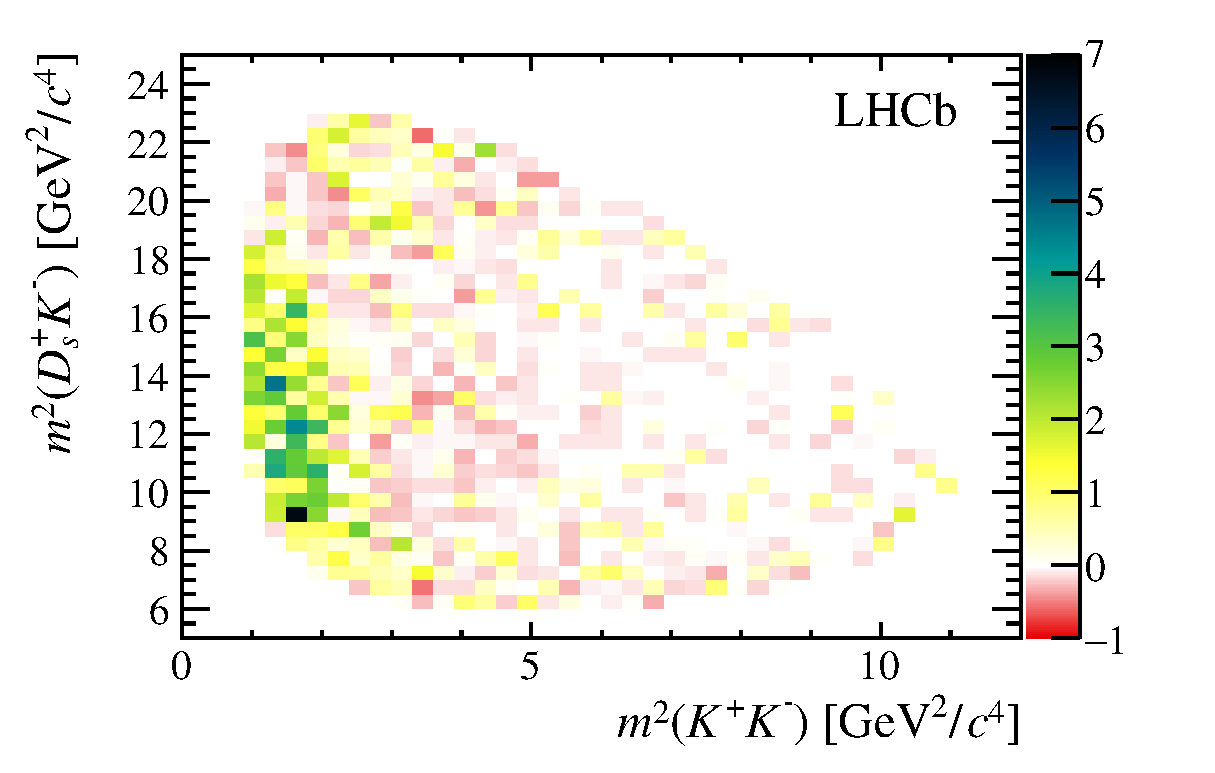
\includegraphics[width=0.8\textwidth]{figs/B2DsKK/Dalitz_plot_sweighted.eps}
    \caption{Dalitz plot}
    \label{fig:B2DsKK_Dalitzplot}   
\end{figure}
%%%%%%%%%%%%%%%%%%%%%%%%%%%%%%%%%%%%%%%%%%%%%%%%%%%%%%%%%%

%%%%%%%%%%%%%%%%%%%%%%%%%%%%%%%%%%%%%%%%%%%%%%%%%%%%%%%%%%
\begin{figure}[!h]
    \centering
    \begin{subfigure}[t]{0.49\textwidth}
        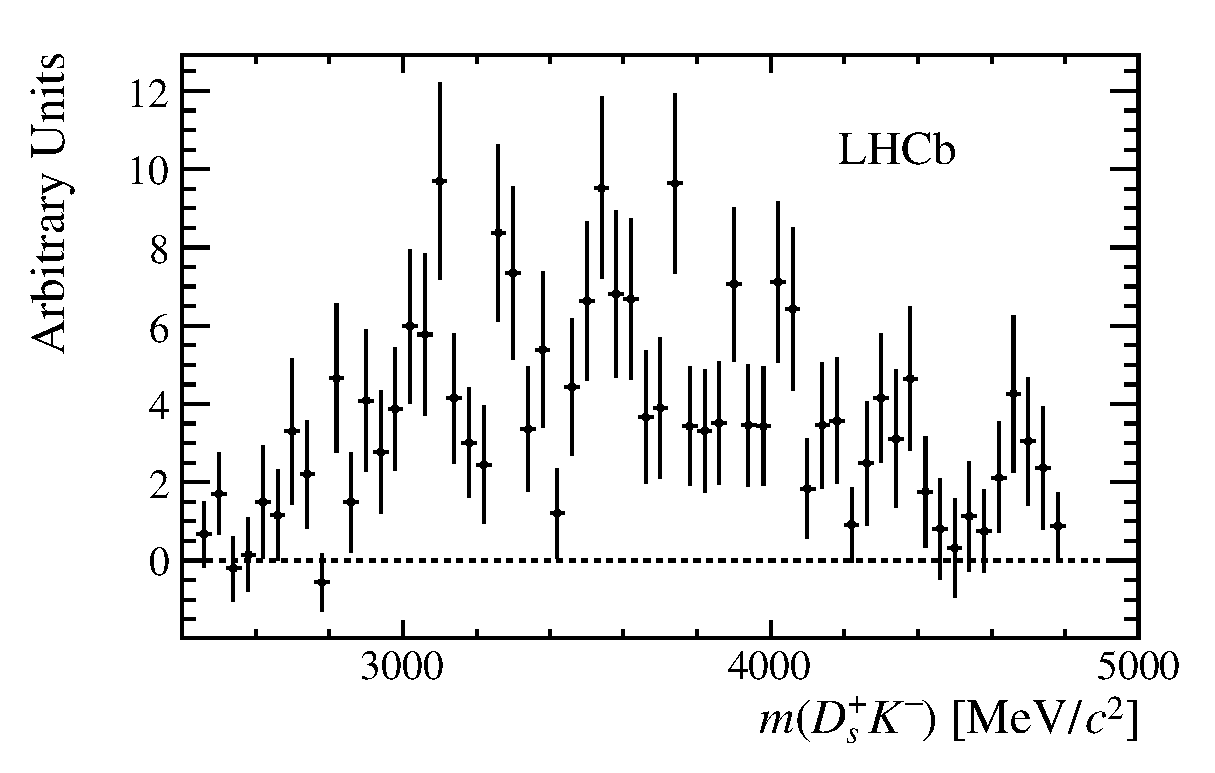
\includegraphics[width=1.0\textwidth]{figs/B2DsKK/DsKm_mass_sweighted.eps}
        %\caption{Normalisation without selection}
    \end{subfigure}
    \begin{subfigure}[t]{0.49\textwidth}
        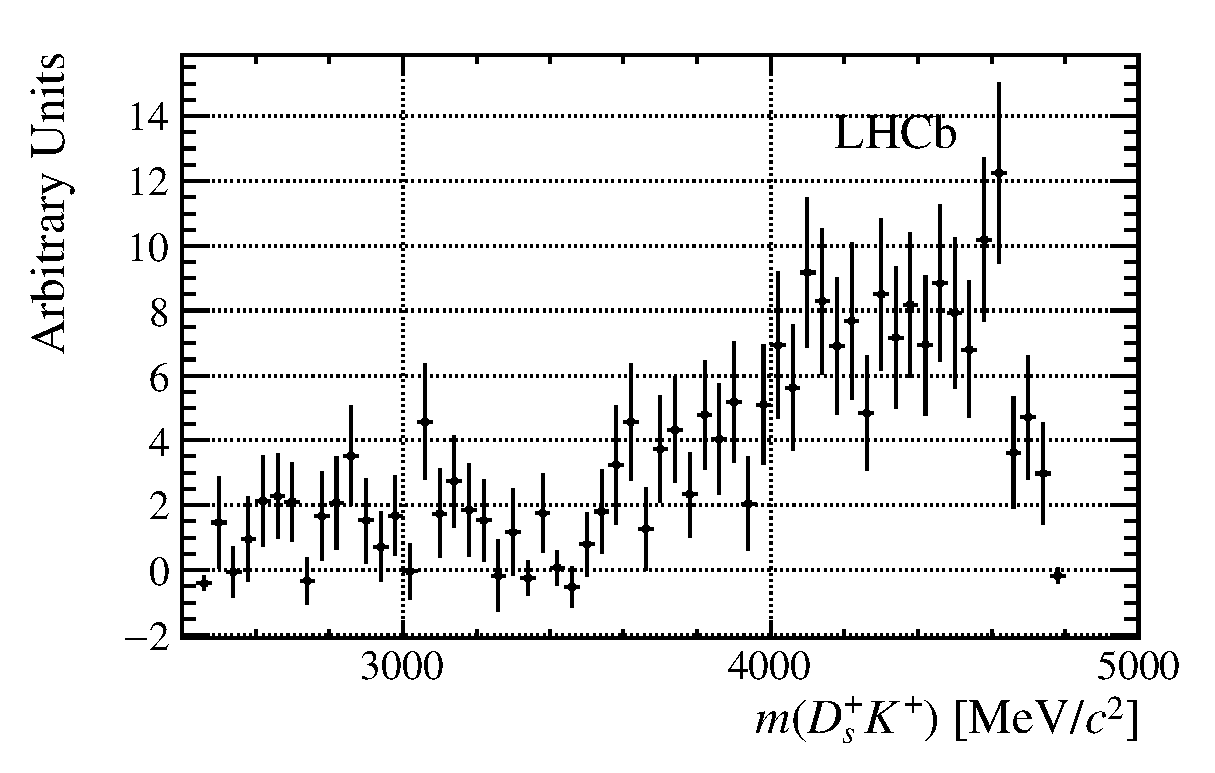
\includegraphics[width=1.0\textwidth]{figs/B2DsKK/DsKp_mass_sweighted.eps}
        %\caption{Normalisation without selection}
    \end{subfigure}
    \begin{subfigure}[t]{0.49\textwidth}
        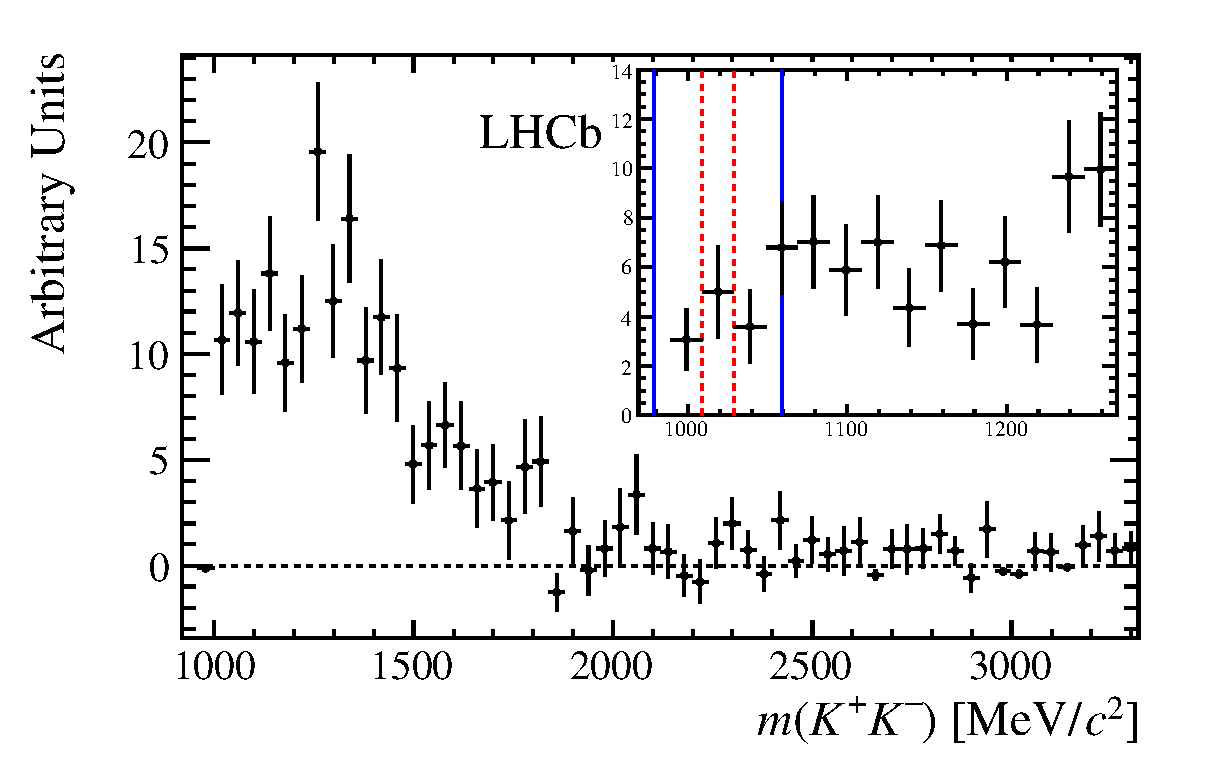
\includegraphics[width=1.0\textwidth]{figs/B2DsKK/phi_mass_sweighted.eps}
        %\caption{Normalisation without selection}
    \end{subfigure}
    \caption{Two-body mass projections}
    \label{fig:B2DsKK_twobodyprojections}
\end{figure}
%%%%%%%%%%%%%%%%%%%%%%%%%%%%%%%%%%%%%%%%%%%%%%%%%%%%%%%%%%

{\color{Red}
\begin{itemize}
\item remove grid from DsKp plot 
\end{itemize}
}

\section{Discussion}
